\documentclass{article}
\usepackage[utf8]{inputenc}
\usepackage[T1]{fontenc}
\usepackage[english]{babel}
\setlength{\parindent}{0pt}
\usepackage{hyperref}
\hypersetup{
    colorlinks=true,
    linkcolor=blue,
    filecolor=magenta,      
    urlcolor=cyan}
\usepackage{graphicx}
\graphicspath{ {./pic/} }
\usepackage{multicol}
\usepackage{lscape}

\usepackage{fourier,amssymb,microtype,amsmath,gensymb}
\newcommand{\R}{\mathbb{R}}
\usepackage{mdframed,caption,xcolor}
\usepackage{tikz,tkz-euclide}

\title{Seminar 12. Auctions and previous exam problems}
\author{Xiaoguang Ling \\  \href{xiaoguang.ling@econ.uio.no}{xiaoguang.ling@econ.uio.no}}
\date{\today}

\begin{document}

\maketitle

%%%%%%%%%%%%%%%%%%%%%%%%%%%%%%%%%%%%%%%%%%%%%%%%%%%%%%%%%%%%%%%%%%%%%%%%%%%%%%%%%%%%%%%%%%%%%%
\begin{mdframed}[backgroundcolor=blue!20,linecolor=white]

The following review part is based on Jehle \& Reny pp.428-432 

\section*{First-price sealed-bid auction}

There are $N$ bidders in an auction, and any bidder $i$ has a private value $v_i$ for the auctioned good. Bidder $i$ can submit any sealed bid $b_i$. We define the bid that can maximize the bidder's payoff (best response) as $b_i^* = \hat{b}(v_i)$. We assume
\begin{itemize}
\item Private value $v_i$ is independent among the bidders; the CDF of $v_i$ is $F(x)$
\item Best response bidding function $\hat{b}(\cdot)$ is strictly increasing and identical for all bidders (we want to find a symmetric NE).
\end{itemize}

\subsection*{What is the BR $\hat{b}(v_i)$ for bidder $i$ ?}

If bidder $i$ with $v_i=r$ submits a price higher than bidder $1$, we must have:

$$\hat{b}(v_1) < \hat{b}(r) \iff v_1  < r, i \neq 1
$$

\medskip

Therefore bidder $i$ can guess how likely he/she defeats bidder $1$, $$Pr\{\text{bidder $i$ defeats bidder 1}\} = Pr\{v_1  < r\} = F(r)$$

and similarly,

$$Pr\{\text{bidder $i$ defeats all the other N-1 bidders}\} = F^{(N-1)}(r)$$


Here is another interesting way to understand function $F^{(N-1)}(x)$:

\smallskip 

Since ``\textit{bidder $i$ defeats all the other N-1 bidders}'' $\iff$ ``\textit{bidder $i$ defeats the bidder with the second-highest private value}'', if we denote the second-highest private value as $\theta$, we can also write the probability above as

\begin{equation}
Pr\{\theta < r\} = F^{(N-1)}(r)
    \label{eq:second}   
\end{equation}

We find that  $F^{(N-1)}(x)$ is actually the CDF of $\theta$! We will use the conclusion later in equation \ref{eq:b}.

\medskip

The maximized expected utility function of bidder $i$ is:
\begin{align*}
u(r)&= Pr\{\text{bidder $i$ defeats all the other N-1 bidders}\} \times (r-\hat{b}(r)) \\&+  Pr\{\text{bidder $i$ lose the auction}\} \times 0 \\ 
&= F^{(N-1)}(r) (r-\hat{b}(r)) + (1-F^{(N-1)}(r))\times 0 \\
&= F^{(N-1)}(r) (r-\hat{b}(r))
\end{align*}

(To calculate $\hat{b}(\cdot)$) Imagine the real private value of bidder $i$ is actually $v$, not $r$, but the bidder reacted (by mistake) as if his/her private value was $r$, i.e. bid at $\hat{b}(r)$ instead of $\hat{b}(v)$. When the bidder realized the mistake, the price had already been submitted...

\medskip

The expected utility function due to the mistake is (eq. 9.1, Jehle \& Reny pp.430):
\begin{align*}
u(r,v)= F^{(N-1)}(r) (v-\hat{b}(r))
\end{align*}

We know only when the wrong private value $r$ is luckily the same as the real private value $v$, will the expected payoff be maximized (since $\hat{b}(v)$ instead of $\hat{b}(r)$ is the best response). That is to say, $r=v$ solves $\max_{r} u(r,v)$.

\medskip

The FOC of $\max_{r} u(r,v)$ is (eq. 9.2, Jehle \& Reny pp.430):

$$\frac{d F^{(N-1)}(r)(v-\hat{b}(r))}{d r} = (N-1)F^{N-2}(r)f(r)(v-\hat{b}(r))-F^{(N-1)}(r)\hat{b}'(r)=0$$

Since $r=v$ solves $\max_{r} u(r,v)$, it must solve the FOC above, i.e. (eq. 9.3, Jehle \& Reny pp.430)

$$(N-1)F(v)^{N-2}f(v)(v-\hat{b}(v))-F^{(N-1)}(v)\hat{b}'(v)=0$$

Which gives,
\begin{align*}
(N-1)F(v)^{N-2}f(v)\hat{b}(v))+ F^{(N-1)}(v)\hat{b}'(v) &= (N-1)F(v)^{N-2}vf(v) \\
\text{(If we treat $v$ as a variable:)} \quad \frac{d F^{(N-1)}(v)\hat{b}(v)}{d v} &= (N-1)F(v)^{N-2}vf(v) \\
F^{(N-1)}(v)\hat{b}(v)&= \int_0^{v} (N-1)F^{(N-2)}(x)xf(x)dx + C
\end{align*}

($C$ is constant)

\medskip

Since a bidder with $v=0$ must bid $0$ to maximize the expected payoff, we know $\hat{b}(0)=0$ in the NE.
\begin{align*}
F(0)^{N-1}\hat{b}(0)&= \int_0^{0} (N-1)F^{(N-2)}(x)xf(x)dx + C \\
0&= 0+ C
\end{align*}

Thus,
\begin{align*}
F^{(N-1)}(v)\hat{b}(v)&= \int_0^{v} (N-1)F^{(N-2)}(x)xf(x)dx \\
\Rightarrow \quad \hat{b}(v)&= \frac{\int_0^{v} (N-1)F^{(N-2)}(x)xf(x)dx}{F^{(N-1)}(v)} \\
&= \frac{\int_0^{v} xdF^{(N-1)}(x)}{F^{(N-1)}(v)} \\
&= \frac{1}{F^{(N-1)}(v)} \int_0^{v}x d F^{(N-1)}(x) \quad \quad (eq.9.5)  \\
&= \int_0^{v}xd\frac{F^{(N-1)}(x)}{F^{(N-1)}(v)}
\end{align*}

\subsection*{$\hat{b}(v)$ as the conditional expectation}

Recall that in Seminar 11, we already know: for a random variable $\theta \in [a,b] \subset \R_1$ and $m \in (a,b)$,

$$E(\theta|\theta \le m) = \int^m_a x d F(x|\theta \le m)=\int^m_a x d \frac{F(x)}{F(m)}$$

where $F(x) = Pr(\theta\le x)$ is the CDF of $\theta$.

\medskip

$\hat{b}(v)$ is actually an expectation of some variable $\theta$ conditional on $\theta \le v$, and the variable $\theta$'s CDF is $Pr(\theta \le x) = F^{(N-1)}(x)$. In equation \ref{eq:second} we already showed $\theta$ is actually the second highest private value.

\medskip

In conclusion, the the BR of any bidder $i$ with private value $v$, is the expectation of the second highest private value conditional on $v$ is higher than the second highest private value (i.e. bidder $i$ wins):
\begin{equation}
\hat{b}(v) = E(\theta|\theta \le v)
    \label{eq:b}   
\end{equation}

\end{mdframed}

\newpage

\section{Jehle \& Reny pp.484, exercise 9.2}

Show in two ways that the symmetric equilibrium bidding strategy of a first-price auction with $N$
symmetric bidders each with values distributed according to $F$, can be written as


$$\hat{b}(v) = v -\int_{0}^{v} \left(\frac{F(x)}{F(v)}\right)^{N-1} dx$$

For the first way, use our solution from the text and apply integration by parts. For the second
way, use the fact that $F^{N-1}(r)(v - \hat{b}(r))$ is maximised in r when $r = v$ and then apply the envelope
theorem to conclude that $d(F^{N-1}(v)(v - \hat{b}(v))/dv = F^{N-1}(v)$; now integrate both sides from $0$ to $v$.

\subsection*{Method 1: Integration by parts}

\begin{mdframed}[backgroundcolor=blue!20,linecolor=white]
Integration by parts: 
$$\int_a^b u(x) \cdot v'(x) dx = \left[u(x) \cdot v(x)\right]_a^b - \int_a^b u'(x) \cdot v(x) dx $$
\end{mdframed}

We start from the euqation above equation (9.5) on Jehle \& Reny pp.431, let's call it equation \ref{eq:95},
\begin{equation}
\hat{b}(v)= \frac{(N-1)}{F^{(N-1)}(v)} \int_0^{v}xf(x)F^{(N-2)}(x)dx
\label{eq:95}   
\end{equation}

Denote,
\begin{equation}
    \begin{cases}
u(x)=x  \\
v(x)= \frac{F^{(N-1)}(x)}{(N-1)}
    \end{cases}
\Rightarrow
	\begin{cases}
 u'(x)= 1 \\
 v'(x)= F^{(N-2)}(x)f(x)
	\end{cases}
\nonumber
\end{equation}

Equation \ref{eq:95} can be rewritten as,
\begin{align*}
\hat{b}(v)&= \frac{(N-1)}{F^{(N-1)}(v)} \int_0^{v}xf(x)F^{(N-2)}(x)dx \\
&= \frac{(N-1)}{F^{(N-1)}(v)} \int_0^{v} u(x)\cdot v'(x)dx \\
\text{(Integration by parts:)}\quad &=\frac{(N-1)}{F^{(N-1)}(v)} \left\{\left[u(x) \cdot v(x)\right]_0^v - \int_0^v u'(x) \cdot v(x) dx\right\} \\
&=\frac{(N-1)}{F^{(N-1)}(v)}  \left\{\left[x \cdot \frac{F^{(N-1)}(x)}{(N-1)}\right]_0^v - \int_0^v 1 \cdot \frac{F^{(N-1)}(x)}{(N-1)} dx \right\} \\
&=\frac{(N-1)}{F^{(N-1)}(v)}  \left\{v \cdot \frac{F^{(N-1)}(v)}{(N-1)} -   \frac{1}{N-1} \int_0^v F^{(N-1)}(x) dx \right\} \\
&= v -  \int_0^v \left[\frac{F(x)}{F(v)}\right]^{(N-1)} dx 
\end{align*}

\subsection*{Method 2: Envelop theorem}


\begin{mdframed}[backgroundcolor=blue!20,linecolor=white]
Envelop theorem (unconstraint case):

\medskip

$f(x;a)$ is a function of $x$ with $a$ as paratmeter. Given any $a$, let $x^*$ be the solution maximizing or minimizing object function $f(x,a)$, i.e. $\max_{x} f(x,a)= f(x^*,a)$, then

$$\frac{d f(x^*,a)}{d a} = \frac{f(x,a)}{d a} \bigg\rvert_{x=x^*} $$
\end{mdframed}

We start from euqation (9.1) on Jehle \& Reny pp.430 (the one called as \textit{``expected utility function due to the mistake''} in the review part),
\begin{align*}
u(r,v)= F^{(N-1)}(r) (v-\hat{b}(r))
\end{align*}

We know $r^*=v$ maximizes $u(r,v)$, i.e. 
\begin{equation}
\max_r u(r,v) = u(r^*,v)=F^{(N-1)}(v) (v-\hat{b}(v))
    \label{eq:max1}   
\end{equation}

On the other hand, by envelop theorem,
\begin{align*}
\frac{d u(r^*,v)}{d v} &= \frac{f(r,v)}{d v} \bigg\rvert_{r=v} \\
&= F^{(N-1)}(r) \bigg\rvert_{r=v} \\
&=F^{(N-1)}(v)
\end{align*}

we find another way to express $u(r^*,v)$:
\begin{equation}
u(r^*,v) = \int_0^v F^{(N-1)}(x) dx + C
    \label{eq:max2}   
\end{equation}

($C=0$ since $u(v=0) =0 = 0 +C$)

Therefore, by equation \ref{eq:max1} and equation \ref{eq:max2},
\begin{align*}
F^{(N-1)}(v) (v-\hat{b}(v)) &= \int_0^v F^{(N-1)}(x) dx \\
\hat{b}(v)&= v - \int_0^v \left[\frac{F(x)}{F(v)}\right]^{(N-1)} dx 
\end{align*}

%%%%%%%%%%%%%%%%%%%%%%%%%%%%%%%%%%%%%%%%%%%%%%%%%%%%%%%%%%%%%%%%%%%%%%%%%%%%%%%%%%%%%%%%%%%%%%

\section{Jehle \& Reny pp.484, exercise 9.1 - Show that the bidding strategy in (9.5) is strictly increasing.}

By exercise 9.1 we know,
$$\hat{b}(v) = v - \frac{\int_0^v F^{N-1}(x) dx}{F^{N-1}(v)} \, .$$

Then:

\begin{align*}
  \frac{d}{dv}\left( \hat{b}(v) \right) &= \frac{d}{dv}\left( v - \frac{\int_0^v F^{N-1}(x) dx}{F^{N-1}(v)} \right) \\
  &= 1 - \frac{\frac{\int_0^vF^{N-1}(x) dx }{dv} \cdot [F^{N-1}(v)]- \left[\int_0^v[F^{N-1}(x)] dx \right] \cdot \frac{F^{N-1}(v)}{dv}}{\left[F^{N-1}(v)\right]^2}\\
  &= 1 - \frac{F^{N-1}(v) \cdot [F^{N-1}(v)] - \left[\int_0^v[F^{N-1}(x)] dx \right] \cdot [(N-1) F^{N-2}(v) f(v)]} {F^{2N-2}(v)} \\
  &= 1 - 1 + \frac{\left[\int_0^v[F^{N-1}(x)] dx \right] \cdot [(N-1) f(v)]} {F^{N}(v)} \\
  &= \frac{\left[\int_0^v[F^{N-1}(x)] dx \right] \cdot [(N-1) f(v)]} {F^{N}(v)}
\end{align*}

If we assume $F(x)$ is strictly increasing and $N > 1$, then $\hat{b}(v) > 0$.

\section{Jehle \& Reny pp.485, exercise 9.3}

This exercise will guide you through the proof that the bidding function in (9.5) is in fact a symmetric
equilibrium of the first-price auction.
%***************************************************

\subsection*{(a) Another way to write the derivative} 

Recall from (9.2) that
$$\frac{du(r,v)}{dr}=(N-1)F^{N-2}(r)f(r)(v-\hat{b}(r))-\textcolor{blue}{F^{N-1}(r)\hat{b'}(r)}.$$
Using (9.3), show that
\begin{align*}
\frac{du(r,v)}{dr}&=(N-1)F^{N-2}(r)f(r)(v-\hat{b}(r))-(N-1)F^{N-2}(r)f(r)(r-\hat{b'}(r)) \\
&= (N-1)F^{N-2}(r)f(r)(v-r)
\end{align*}

\medskip

\begin{mdframed}[backgroundcolor=blue!20,linecolor=white]
Equation 9.3 on Jehle \& Reny pp.430 is,
$$(N-1)F(v)^{N-2}f(v)\hat{b}(v))+ \textcolor{blue}{F^{(N-1)}(v)\hat{b}'(v)} = (N-1)F(v)^{N-2}vf(v) $$
\end{mdframed}

Equation 9.3 holds for any $v$, since $v$ is the variable. It will also hold if we take $v=r$, i.e.

$$(N-1)F^{N-2}(r)f(r)\hat{b}(r))+ \textcolor{blue}{F^{(N-1)}(r)\hat{b}'(r)} = (N-1)F^{N-2}(r)rf(r) $$
which yields,
\begin{align*}
\textcolor{blue}{F^{(N-1)}(r)\hat{b}'(r)} &= (N-1)F^{N-2}(r)rf(r)-(N-1)F^{N-2}(r)f(r)\hat{b}(r)) \\
&=(N-1)F^{N-2}(r)f(r)\left[r - \hat{b}(r)\right]
\end{align*}

Substituting the result above into equation 9.2 yields,
\begin{align*}
\frac{du(r,v)}{dr}&=(N-1)F^{N-2}(r)f(r)(v-\hat{b}(r))-\textcolor{blue}{F^{N-1}(r)\hat{b'}(r)} \\
&=(N-1)F^{N-2}(r)f(r)(v-\hat{b}(r))-(N-1)F^{N-2}(r)f(r)\left[r - \hat{b}(r)\right] \\
&= (N-1)F^{N-2}(r)f(r)(v-r)
\end{align*}



%***************************************************

\subsection*{(b) Minimum or maximum?}Use the result in part (a) to conclude that $du(r, v)/dr$ is positive when $r < v$ and negative when
$r > v$, so that $u(r, v)$ is maximised when $r = v$.

\bigskip

$$\frac{du(r,v)}{dr} = (N-1)F^{N-2}(r)f(r)(v-r)$$

Obviously, if we assume $F(x)$ is strictly increasing and $N>1$,
 $\frac{du(r,v)}{dr} > 0$ when $r < v$ and $\frac{du(r,v)}{dr} < 0$ when
$r > v$. Therefore $r=v$ maximizes $u(r,v)$.



%%%%%%%%%%%%%%%%%%%%%%%%%%%%%%%%%%%%%%%%%%%%%%%%%%%%%%%%%%%%%%%%%%%%%%%%%%%%%%%%%%%%%%%%%%%%%%

\section{Problems 2  of the exam in \href{https://www.uio.no/studier/emner/sv/oekonomi/ECON4240/previous-exams/}{ECON4240, Spring 2005}}

Consider a strategic situation between an employer ($E$) and a worker ($W$). $E$ can either accept
($A$) or reject ($R$) $W$. $W$ can either become skilled ($S$) through education, or remain unskilled
($U$). $W$ can be of two types; either he is inherently high ability ($H$) or he is inherently low
ability ($L$). The players' payoffs depending on their actions and W's type is shown below.

{\centering
\includegraphics[width=0.8\textwidth]{12.q2}
\vspace{2mm}}

%***************************************************

\subsection*{a) Rationalizable strategies \& NE} For each of these games, determine the set of (pure) rationalizable strategies for each
player, and the set of pure-strategy Nash equilibria.

\bigskip

In Game $H$: Only $A$ and $S$ are rationalizable. $(A, S)$ is the unique NE. 

In Game $L$. Only $R$ and $U$ are rationalizable. $(R, U)$ is the unique NE.


\subsection*{b) Bayesian normal form} Assume next that only $W$ knows his own type, while player $E$ thinks that the two types
of $W$ are equally likely. Model this situation in an ex ante perspective by specifying
the Bayesian normal form.

\bigskip

Denote the Worker's contingent choices are: If Game $H$, $S$ and $U$; If Game $L$, $S'$ and $U'$. The Baysian normal form is:


\begin{center}
\includegraphics[width=0.6\textwidth]{12.q2_2}
\vspace{2mm}
\end{center}

%***************************************************

\subsection*{c) Rationalizable strategy \& BNE} For the Bayesian normal form found in part (b), determine the set of (pure)
rationalizable strategies for each player, and the set of pure-strategy and/or mixedstrategy Nash equilibria.

\bigskip

\begin{center}
\includegraphics[width=0.6\textwidth]{12.q2_3}
\vspace{2mm}
\end{center}


\textbf{(1) Rationalizable strategy}

\medskip

For the Employer, both $A$ and $R$ are rationalizable.

\medskip

For the Worker, $US'$ is dominated by $SS'$; $UU'$ is dominated by $SU'$. The rationalizable strategies are $SS'$ and $SU'$.

\medskip

\textbf{(2) Pure-strategy NE}

$$(A,SS'),(R,SU')$$

\smallskip

\textbf{(3) Mixed-strategy NE}

\medskip

Since $US'$ and $UU'$ are dominated, the Employer believes the Worker will choose 
them with probability (0,0).

\medskip

The Employer believes the Worker chooses $SS'$ and $SU'$ with probability $(p,1-p)$;
The Worker believe the Employer chooses $A$ and $R$ with probability $(q,1-q)$.

$$E(U^E_A) = p \times 0.5 + (1-p) \times (-0.5) = p-0.5$$
$$E(U^E_R) = p \times 0 + (1-p) \times 0 = 0$$
$$E(U^E_A) = E(U^E_R) \Rightarrow p=0.5$$


$$E(U^W_{SS'}) = q \times 1 + (1-q) \times (-1) = 2q-1$$
$$E(U^W_{SU'}) = q \times 0.5 + (1-q) \times 0.5 = 0.5$$
$$E(U^W_{SS'}) = E(U^W_{SU'}) \Rightarrow 2q-1=0.5 \Rightarrow \tfrac34$$

The Mixed-strategy NE is: the Employer chooses $A$ and $R$ with probability $(\tfrac34,\tfrac14)$; Worker chooses $SS'$ and $SU'$ with probability $(0.5,0.5)$, i.e.

$$\{(\tfrac34,\tfrac14), (0.5,0.5,0,0)\}$$

%%%%%%%%%%%%%%%%%%%%%%%%%%%%%%%%%%%%%%%%%%%%%%%%%%%%%%%%%%%%%%%%%%%%%%%%%%%%%%%%%%%%%%%%%%%%%%

\section{Problems 3  of the exam in \href{https://www.uio.no/studier/emner/sv/oekonomi/ECON4240/previous-exams/}{ECON4240, Spring 2005}}

Problem 3 (20 \%)
Consider again the strategic situation between an employer ($E$) and a worker ($W$) described in
Problem 2. Assume (as in parts b and c) of Problem 2) that only $W$ knows his own type, while
player $E$ thinks that the two types of $W$ are equally likely.
%***************************************************

\subsection*{a) (Screening)} Assume now that $E$ acts before W, and that $E$'s choice of A or R can be
observed by $W$ before he makes his choice of $S$ or $U$. Show that there is a unique
subgame perfect Nash equilibrium.

\medskip

\textbf{Extensive Form:}

\begin{center}
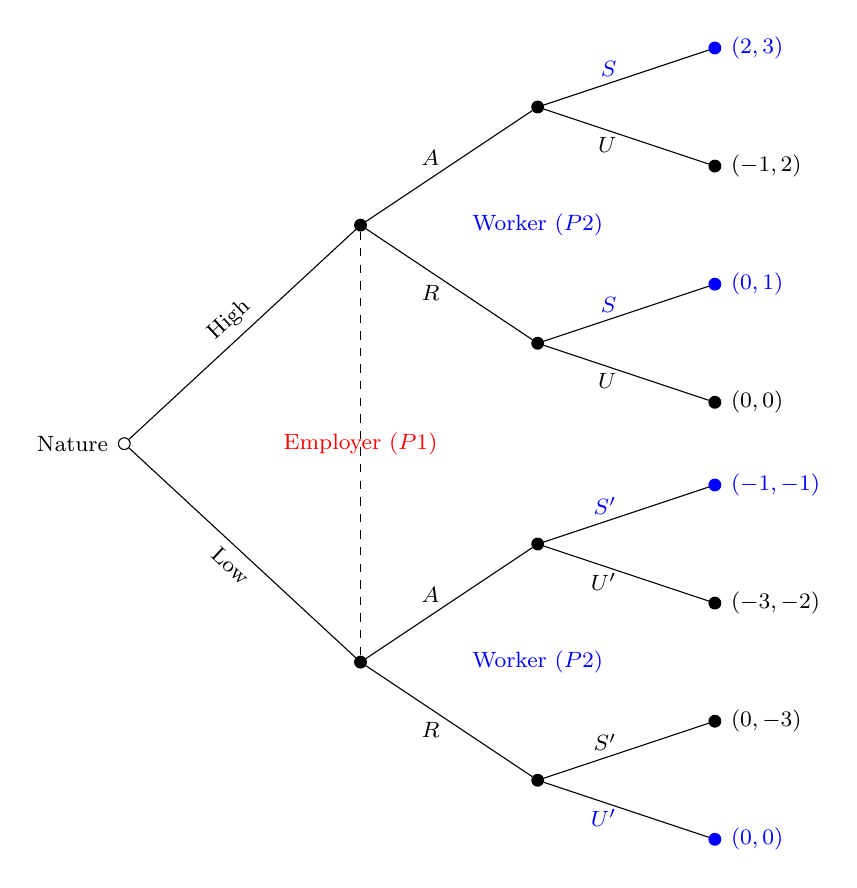
\begin{tikzpicture}[scale=1.5,font=\footnotesize]
\tikzset{
% Two node styles for game trees: solid and hollow
solid node/.style={circle,draw,inner sep=1.5,fill=black},
hollow node/.style={circle,draw,inner sep=1.5}
}
% Specify spacing for each level of the tree
\tikzstyle{level 1}=[level distance=20mm,sibling distance=37mm]
\tikzstyle{level 2}=[level distance=15mm,sibling distance=20mm]
\tikzstyle{level 3}=[level distance=15mm,sibling distance=10mm]
\tikzstyle arrowstyle=[scale=1]
\tikzstyle directed=[postaction={decorate,decoration={markings,
mark=at position .5 with {\arrow[arrowstyle]{stealth}}}}]

% The Tree
\node(0)[hollow node,label=left:{Nature}]{}[grow=east]
child{node(1)[solid node]{}
child{node(3)[solid node]{}
child{node[solid node,blue,label=right:{\textcolor{blue}{$(0,0)$}}]{}edge from parent node[left,blue,yshift=-3]{$U'$}}
child{node[solid node,label=right:{$(0,-3)$}]{}edge from parent node[left,yshift=3]{$S'$}}
edge from parent node[left,yshift=-3]{$R$}}
child{node(4)[solid node]{}
child{node[solid node,label=right:{$(-3,-2)$}]{}edge from parent node[left,yshift=-3]{$U'$}}
child{node[solid node,blue,label=right:{\textcolor{blue}{$(-1,-1)$}}]{}edge from parent node[left,blue,yshift=3]{$S'$}}
edge from parent node[left,yshift=3]{$A$}
}
edge from parent node [midway, below, sloped] (TextNode) {Low}
}
child{node(2)[solid node]{}
child{node(5)[solid node]{}
child{node[solid node,label=right:{$(0,0)$}]{}edge from parent node[left,yshift=-3]{$U$}}
child{node[solid node,blue,label=right:{\textcolor{blue}{$(0,1)$}}]{}edge from parent node[left,blue,yshift=3]{$S$}}
edge from parent node[left,yshift=-3]{$R$}}
child{node(6)[solid node]{}
child{node[solid node,label=right:{$(-1,2)$}]{}edge from parent node[left,yshift=-3]{$U$}}
child{node[solid node,blue,label=right:{\textcolor{blue}{$(2,3)$}}]{}edge from parent node[left,blue,yshift=3]{$S$}}
edge from parent node[left,yshift=3]{$A$}
}
edge from parent node [midway, above, sloped] (TextNode) {High}
};
% information set
\draw [dashed] (2) -- (1) ;
% specify mover
\node at ($(1)!.5!(2)$) {\textcolor{red}{Employer ($P1$)}};
\node at ($(5)!.5!(6)$) {\textcolor{blue}{Worker ($P2$)}};
\node at ($(3)!.5!(4)$) {\textcolor{blue}{Worker ($P2$)}};
\end{tikzpicture}
\end{center}

\medskip

The strategy of the $Worker$:
\begin{itemize}
\item If High:
\begin{itemize}
\item when $E$ chooses $A$, $W$ chooses $S$
\item when $E$ chooses $R$, $W$ chooses $S$
\end{itemize}
\item If Low:
\begin{itemize}
\item when $E$ chooses $A$, $W$ chooses $S'$
\item when $E$ chooses $R$, $W$ chooses $U'$
\end{itemize}
\end{itemize}

For the $Employer$:

$$E(U^E_A) = \tfrac12 \times 2 +\tfrac12 \times (-1) = 0.5$$
$$E(U^E_R) = \tfrac12 \times 0 +\tfrac12 \times 0 = 0$$
$$\Rightarrow E(U^E_A) > E(U^E_R)$$

The strategy of the $Employer$ is to choose $A$.

\medskip

Therefore there is a SPNE:

\{(For High ability Worker:) $S$ after $A$, $S$ after $R$. (For Low ability Worker:) $S'$ after $A$, $U'$ after $R$ ; (For Employer) $A$\}

%***************************************************

\subsection*{b) (Signaling)} Assume now that $W$ acts before $E$, and that $W$'s choice of $S$ or $U$ can be
observed by $E$ before she makes her choice of $A$ or $R$. Show that there is a unique
perfect Bayesian equilibrium.

\medskip

\textbf{Extensive Form:}

\medskip

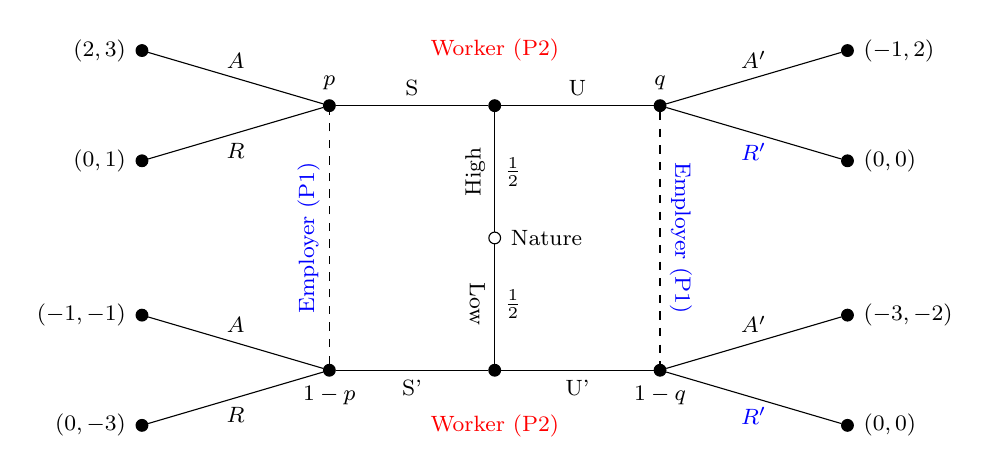
\begin{tikzpicture}[scale=1.4,font=\footnotesize]
\tikzset{
% Two node styles for game trees: solid and solid
solid node/.style={circle,draw,inner sep=1.5,fill=black},
hollow node/.style={circle,draw,inner sep=1.5}}
% Specify spacing for each level of the tree
\tikzstyle{level 1}=[level distance=12mm,sibling distance=25mm]
\tikzstyle{level 2}=[level distance=15mm,sibling distance=15mm]
\tikzstyle{level 3}=[level distance=17mm,sibling distance=10mm]
% The Tree
\node(0)[hollow node,label=right:{Nature}]{}
child[grow=up]{node[solid node,label=above:{
\begin{tabular}{c}
\textcolor{red}{Worker (P2)} \\ \\
\end{tabular}}] {}
child[grow=left]{node(1)[solid node,label=above:{$p$}]{}
child{node[solid node,label=left:{$(2,3)$}]{} edge from parent node [above]{$A$}}
child{node[solid node,label=left:{$(0,1)$}]{} edge from parent node [below]{$R$}}
edge from parent node [above]{S}}
child[grow=right]{node(3)[solid node,label=above:{$q$}]{}
child{node[solid node,label=right:{$(0,0)$}]{} edge from parent node [below]{\textcolor{blue}{$R'$}}}
child{node[solid node,label=right:{$(-1,2)$}]{} edge from parent node [above]{$A'$}}
edge from parent node [above]{U}
}
edge from parent node [right]{$\tfrac12$} node [midway, above, sloped] (TextNode){High}
}
child[grow=down]{node[solid node,label=below:{\begin{tabular}{c}
\\ \textcolor{red}{Worker (P2)}
\end{tabular}}] {}
child[grow=left]{node(2)[solid node,label=below:{$1-p$}]{}
child{node[solid node,label=left:{$(-1,-1)$}]{} edge from parent node [above]{$A$}}
child{node[solid node,label=left:{$(0,-3)$}]{} edge from parent node [below]{$R$}}
edge from parent node [below]{S'}
}
child[grow=right]{node(4)[solid node,label=below:{$1-q$}]{}
child{node[solid node,label=right:{$(0,0)$}]{} edge from parent node [below]{\textcolor{blue}{$R'$}}}
child{node[solid node,label=right:{$(-3,-2)$}]{} edge from parent node [above]{$A'$}}
edge from parent node [below]{U'}
}
edge from parent node [right]{$\tfrac12$} node[midway, below, sloped] (TextNode){Low}
};
% information set
\draw [dashed] (2) -- (1) node [midway, above, sloped, blue] (TextNode) {Employer (P1)};
\draw [dashed] (3) -- (4) node [midway, above, sloped, blue] (TextNode) {Employer (P1)};
\end{tikzpicture}


\medskip

The Worker has 4 possible strategies: $SS',UU',SU',US'$. 

\smallskip

Denote the updated belief of the Employer :
\begin{itemize}
\item $Pr(\text{Strong} | P/P') = p$
\item $Pr(\text{Weak} | U/U') = q$
\end{itemize}


\textbf{(1) When the Employer believes the Worker chooses $SS'$}

Then $p=Pr(\text{High})=0.5$,

$$E[U^E_{A}] = 0.5 \times 2+ 0.5\times (-1) = 0.5$$
$$E[U^E_{R}] = 0.5 \times 0+ 0.5 \times 0 = 0$$
$$E[U^E_{A}]>E[U^E_{R}]$$

The BR of the Employer is to choose $A$.

\smallskip

If the Worker surprisingly chooses $U/U'$, we can see that $R'$ dominates $A'$
for the Employer. Therefore, the Low ablility Worker will deviate from $S'$ to $U'$
to have a higher payoff ($U'$ and $R'$ leads to $(0,0)$)

\smallskip

$\Rightarrow SS'$ is not part of a PBE.

\medskip

\textbf{(2) When the Employer believes the Worker chooses $UU'$}

\smallskip

Since $R'$ dominates $A'$, the Employer will always choose $R'$. 
For a High ability Worker, deviating from $U$ to $S$ will always lead to
higher payoff (either 3 or 1), no matter how the Employer reacts.

\smallskip

$\Rightarrow UU'$ is not part of a PBE.

\medskip

\textbf{(3) When the Employer believes the Worker chooses $SU'$}

\smallskip

Then $p=1,q=0$,

\smallskip

The BR of the Employer is to choose $A$ after $S/S'$ (payoff is be $(2,3)$) and $R'$ after $U/U'$(payoff is be $(0,0)$).

\smallskip

If the High ability Worker eviates to $U$, the payoff is $(0,0)$, lower than $(2,3)$;
If the Low ability Worker eviates to $S$, the payoff is $(-1,-1)$, lower than $(0,0)$;

\smallskip

There is no incentive for the Worker to deviate.
$\Rightarrow SU'$ is part of a PBE.

\medskip

\textbf{(4) When the Employer believes the Worker chooses $US'$}

\smallskip

Then $p=0,q=1$,

\smallskip

The BR of the Employer is to choose $R$ after $S/S'$ and $R'$ after $U/U'$.

\smallskip

For a High ability Worker, deviating from $U$ to $S$ will increase the payoff from $(0,0)$ to $(0,1)$.

\smallskip

For a Low ability Worker, deviating from $S'$ to $U'$ will increase the payoff from $(0,-3)$ to $(0,0)$.

\smallskip

$\Rightarrow US'$ is not part of a PBE.

\medskip

In conclusion, there is only one PBE:
$$\{SU',AR',p=1,q=0\}$$



\end{document}
